\documentclass[11pt,a4paper,twoside,openright,bibliography=totoc]{scrbook}

\usepackage{scrhack}
\usepackage{graphicx,xcolor,float}
\usepackage{amssymb,amsmath,array}
\usepackage{varwidth,algpseudocode}

% Color citation, references and links.
\usepackage{url,hyperref}
\hypersetup{
  colorlinks,
  linkcolor={black},
  citecolor={red!70!black},
  urlcolor={blue!70!black}
}
\usepackage[labelfont=bf]{caption} % Bold figure titles.

\renewcommand{\t}{\text} % Shorten \text command.

\begin{document}
% Example of title page for the projects carried out within the lasec 

% Simply include it in your mastex tex file: 
%        % Example of title page for the projects carried out within the lasec 

% Simply include it in your mastex tex file: 
%        % Example of title page for the projects carried out within the lasec 

% Simply include it in your mastex tex file: 
%        \input{cover}


% Updated March 2006 (SP)


\newcommand{\logoepfl}[0]{
  \begin{center}
    
\includegraphics[width=4cm]{cover/logo_epfl_coul.eps}
  \end{center}
  \vspace{0.3cm}
  \hrule
}
\newcommand{\logolasec}[0]{
  \vspace{1cm}
  \hrule
  \begin{center}
    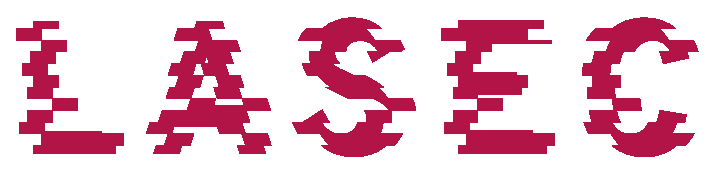
\includegraphics[width=4.5cm]{cover/logo_lasec_coul.eps}
  \end{center}
}
\newcommand{\project}[1]{
  \begin{center}
    \large{#1}
  \end{center}
  \vspace{1cm}
}
\newcommand{\department}[1]{
  \begin{center}
    \large{#1}
  \end{center}
}
\newcommand{\supervisor}[3]{
  \begin{center}
    \begin{normalsize}{
        \bfseries #1}\\#2\\#3
    \end{normalsize}
  \end{center}
}
\renewcommand{\author}[1]{
  \begin{center}
    \Large{#1}
  \end{center}
  \vspace{0.5cm}
}
\renewcommand{\title}[1]{
  \vspace{3cm}
  \begin{center}
    \huge{#1}
  \end{center}
  \vspace{1.7cm}
}
\renewcommand{\date}[2]{
  \begin{center}
    \normalsize{#1 #2}
  \end{center}
  \vspace{0.5cm}
}


\thispagestyle{empty}


% begin title page
\logoepfl

\title{Ratcheting}

\author{Andrea Caforio}
\department{School of Computer and Communication Sciences}
\project{Optional Semester Project}

\date{January}{2019}

\begin{center}
  \begin{tabular}{cc}
    \begin{tabular}{p{4.0cm}}
      \supervisor{Responsible}{Prof. Serge Vaudenay}{EPFL / LASEC}
    \end{tabular}&
    \begin{tabular}{p{4.0cm}}
      \supervisor{Supervisor}{Dr. Betül Durak}{EPFL / LASEC}
    \end{tabular}
  \end{tabular}
\end{center}

\logolasec
% end title page




% Updated March 2006 (SP)


\newcommand{\logoepfl}[0]{
  \begin{center}
    
\includegraphics[width=4cm]{cover/logo_epfl_coul.eps}
  \end{center}
  \vspace{0.3cm}
  \hrule
}
\newcommand{\logolasec}[0]{
  \vspace{1cm}
  \hrule
  \begin{center}
    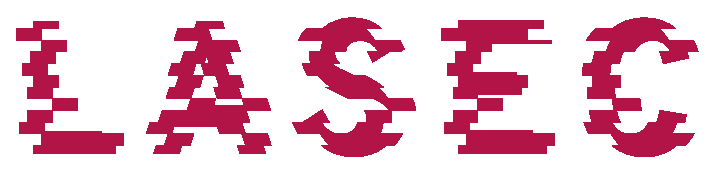
\includegraphics[width=4.5cm]{cover/logo_lasec_coul.eps}
  \end{center}
}
\newcommand{\project}[1]{
  \begin{center}
    \large{#1}
  \end{center}
  \vspace{1cm}
}
\newcommand{\department}[1]{
  \begin{center}
    \large{#1}
  \end{center}
}
\newcommand{\supervisor}[3]{
  \begin{center}
    \begin{normalsize}{
        \bfseries #1}\\#2\\#3
    \end{normalsize}
  \end{center}
}
\renewcommand{\author}[1]{
  \begin{center}
    \Large{#1}
  \end{center}
  \vspace{0.5cm}
}
\renewcommand{\title}[1]{
  \vspace{3cm}
  \begin{center}
    \huge{#1}
  \end{center}
  \vspace{1.7cm}
}
\renewcommand{\date}[2]{
  \begin{center}
    \normalsize{#1 #2}
  \end{center}
  \vspace{0.5cm}
}


\thispagestyle{empty}


% begin title page
\logoepfl

\title{Ratcheting}

\author{Andrea Caforio}
\department{School of Computer and Communication Sciences}
\project{Optional Semester Project}

\date{January}{2019}

\begin{center}
  \begin{tabular}{cc}
    \begin{tabular}{p{4.0cm}}
      \supervisor{Responsible}{Prof. Serge Vaudenay}{EPFL / LASEC}
    \end{tabular}&
    \begin{tabular}{p{4.0cm}}
      \supervisor{Supervisor}{Dr. Betül Durak}{EPFL / LASEC}
    \end{tabular}
  \end{tabular}
\end{center}

\logolasec
% end title page




% Updated March 2006 (SP)


\newcommand{\logoepfl}[0]{
  \begin{center}
    
\includegraphics[width=4cm]{cover/logo_epfl_coul.eps}
  \end{center}
  \vspace{0.3cm}
  \hrule
}
\newcommand{\logolasec}[0]{
  \vspace{1cm}
  \hrule
  \begin{center}
    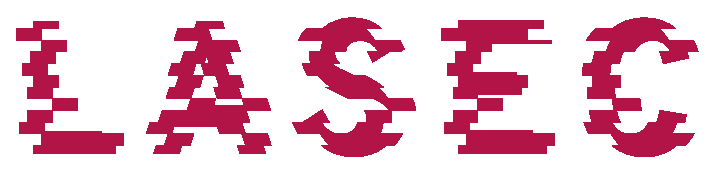
\includegraphics[width=4.5cm]{cover/logo_lasec_coul.eps}
  \end{center}
}
\newcommand{\project}[1]{
  \begin{center}
    \large{#1}
  \end{center}
  \vspace{1cm}
}
\newcommand{\department}[1]{
  \begin{center}
    \large{#1}
  \end{center}
}
\newcommand{\supervisor}[3]{
  \begin{center}
    \begin{normalsize}{
        \bfseries #1}\\#2\\#3
    \end{normalsize}
  \end{center}
}
\renewcommand{\author}[1]{
  \begin{center}
    \Large{#1}
  \end{center}
  \vspace{0.5cm}
}
\renewcommand{\title}[1]{
  \vspace{3cm}
  \begin{center}
    \huge{#1}
  \end{center}
  \vspace{1.7cm}
}
\renewcommand{\date}[2]{
  \begin{center}
    \normalsize{#1 #2}
  \end{center}
  \vspace{0.5cm}
}


\thispagestyle{empty}


% begin title page
\logoepfl

\title{Ratcheting}

\author{Andrea Caforio}
\department{School of Computer and Communication Sciences}
\project{Optional Semester Project}

\date{January}{2019}

\begin{center}
  \begin{tabular}{cc}
    \begin{tabular}{p{4.0cm}}
      \supervisor{Responsible}{Prof. Serge Vaudenay}{EPFL / LASEC}
    \end{tabular}&
    \begin{tabular}{p{4.0cm}}
      \supervisor{Supervisor}{Dr. Betül Durak}{EPFL / LASEC}
    \end{tabular}
  \end{tabular}
\end{center}

\logolasec
% end title page


\tableofcontents

\chapter{Introduction}
\label{chap:introduction}

Messaging has become an ubiquitous resource in the daily lives of
millions of people around the globe through the widespread adoption of
instant messaging applications. The design of protocols which
facilitate securing messaging or key-agreement is faced with a unique
set of challenges, this is due to the longevity of sessions between
communicating parties and the inherently asynchronous notion of
messaging where a participant is both the sender and recipient of
messages and the time a message is sent or received is undefined. In
such a setting the leakage of a state to the adversary is especially
devastating since in a naive protocol it would not only enable him to
recover past messages but also allow future impersonations of the
victim.
Ratcheting has established itself as the go-to technique in
order to mitigate these risks. Akin to its mechanical equivalent the
states are continuously moved forward (updated) without the
possibility of going backwards, i.e.~it should be impossible to
recover past states from the current one.
\begin{figure}[H]
  \centering
  
\includegraphics[scale=0.1]{figures/ratchet-icon.eps}
  \caption{Symbolic Ratchet Wheel}
  \label{fig:ratchet-wheel}
\end{figure}
This further implies that
past message remain secure even in the presence of and adversary who
can expose the state of a participant. The literature labels protocols
that deploy ratchets as \textit{forward-secure}. This technique saw
its inception in 2004 as part of the Off-the-Record messaging
protocol~\cite{borisov2004off}. It only recently gained traction
through the massively popular Signal protocol~\cite{perrin2016double}.
The release of this protocol however predates its first formal
security analysis in 2017~\cite{cohn2017formal}
and since then several novel protocols with various degrees of
security levels have been proposed. Among others
these protocols also attempt the satisfy the notion of \textit{future
secrecy} in which future states and messages remain secure even if the
current state has been leaked. Furthermore, a secure messaging
protocol should be efficient enough to run smoothly even on
computationally inferior devices thus the choice of fast primitives
that do not compromise the promised security levels play a crucial
part in the construction of messaging protocols. Even though on paper
the attained levels of security in these new protocol often only
differ marginally the effects on performance metrics are of a
different kind with sometimes huge differences between the protocols.

% Add some more text here.

\section{Contributions}
\label{sec:contributions}

This project is concerned with surveying and solidifying the
performance differences of six new secure messaging or key-update
protocols that have been proposed during the past two years. In
chapter~\ref{chap:protocols} the notion of secure messaging and
especially ratcheting is formally reviewed before each protocol is
summarized in terms of composition and security levels, then in
chapter~\ref{chap:benchmarks} the protocols are measured and compared
on the basis of several benchmarks. In chapter~\ref{chap:bark} we
extend and modify the in-house Bidirectional Asynchronous Ratcheted
Key Agreement protocol (BARK) proposed by the LASEC laboratory into a
faster version with only minor concessions in terms of security before
concluding this report in the last chapter.

\section{Circumstances}
\label{sec:circumstances}

This project has been conducted as part of the third master semester optional
semester project in computer science course (CS-596) offered by the
School of Computer and Communications Sciences at EPFL and is credited
with eight points. It was supervised by Doctor Betül Durak of
the LASEC laboratory.

\chapter{Protocols}
\label{chap:protocols}

As laid out in the introduction the Signal~\cite{perrin2016double}
protocol created and deployed well before the establishment of a
serious secure messaging definition thus it is lacking any form of
security proof. The subsequent analysis in 2007~\cite{cohn2017formal}
was then more concerned with proving the security of specific Signal
instances than treating the general case of securing
messaging. Formally, ratcheted messaging attempts to satisfy some
correctness and security notions.


\section{Ratcheted Messaging}
\label{sec:ratcheted-messaging}

For the remainder of this text let Alice and Bob be the communicating
parties through an insecure channel. Alice and Bob take on random
roles throughout their communication and are not necessarily
synchronized meaning that the reception of sent messages may be
delayed to a point where there are already new messages in the channel
travelling in the opposite direction. Note that this does not imply
that messages may be dropped or received in a different order than
they were initially sent in, this will be important later on when
the actual protocols are described. Figure % TODO: insert figure here
shows an example asynchronous traffic transcript. The initial states
of Alice and Bob are created and distributed by a trusted party, these
states are updated with each send or receive operation. In the case
of a key-agreement protocol the update information corresponding to
the created key of the sender should generate the same key at
the receiver when the update message is received. Analogous,
for a messaging protocol where a encrypted message should be
correctly deciphered by the receiver upon arrival. In figure
% TODO: insert figure here
for example the message sent by Alice at time $t_0$ is only
received by Bob at time $t_8$ but should nonetheless produce
a correct key or plaintext regardless of the messages sent
by Bob in the meantime that updated Bob's state.

\section{Ratchet Security}
\label{sec:ratchet-security}

These continuous updates of the states are supposed to be irreversible
such that past states may not be derived from any future state thus
yielding forward security protecting past messages from being
compromised. This was the original goal that ratcheting tried to
achieve. Naively, a ratchet can be constructed through the usage of a
one-way function the simply updates the states of the communicating
parties. In practice, a hash-function would be deployed as a
reasonable alternative with the downside of losing the asynchronous
communication property~\cite{bellare2003forward}. On the other hand if
some randomness is included in the creation of an updated state we can
protect future states from being recreated by an adversary after an
exposure yielding future secrecy or post-compromise security. Another
way is the usage of some key-agreement protocol to schedule the
creation of new states between the parties~\cite{cohn2016post}.  Again
both constructions come at the cost of losing asynchronous
communications. Asynchronous communications is thus a challenging
obstacle that significantly complicates the design and analysis
of ratcheted key-agreement or messaging protocols.

\bigskip

The adversary in ratcheted protocols is quite powerful and can be both
passive and to a certain extend active. This means he has access to
the full message transcript, can expose the states of both
participants, corrupt the states or impersonate users and even choose
the randomness used by the participants. As it is usual in such cases
we assess the advantage of any adversary as part of some key (KIND) or
ciphertext (CIND) indistinguishability game where the adversarial
algorithm $\mathcal{A}$ has access to the send and receive procedures
of both Alice and Bob can expose their states and in the end tries to
distinguish some key from random in the KIND game or decide
which one of two chosen messages corresponds to a given ciphertext
in the CIND game.

\begin{figure}[H]
  \centering
  \scalebox{0.9}{%
    \fbox{%
      \algrenewcommand\textproc{}
      \algrenewcommand\algorithmicprocedure{\textbf{Game}}

      \begin{minipage}{.5\linewidth}
        \begin{algorithmic}[1]
          \Procedure{$\t{KIND}_b^\mathcal{A}$}{}
          \State $(\t{st}_\t{A},\t{st}_\t{B}) \gets$ \Call{Init}{$1^\lambda$}
          \State $b' \gets \mathcal{A}^{\t{RATCH,EXP,TEST}}$
          \State \Return $b'$
          \EndProcedure
        \end{algorithmic}
      \end{minipage}

      \vline

      \begin{minipage}{.5\linewidth}
        \begin{algorithmic}[1]
          \Procedure{TEST}{$\t{P}$}
          \If{$b = 1$}
          \State \Return $k_\t{P}$
          \EndIf
          \State \Return random $\{0,1\}^{|k_\t{P}|}$ 
          \EndProcedure

          \item[] % Blank line.

          \Procedure{EXP}{$\t{P}$}
          \State \Return $\t{st}_\t{P}$ 
          \EndProcedure
       \end{algorithmic}
     \end{minipage}%
    }
  }
  \caption{Generic Key-Indistinguishability Game}
  \label{fig:kind}
\end{figure}

Figure~\ref{fig:kind} depicts a generic KIND game where \texttt{RATCH} denotes
the send or receive procedures for both Alice and Bob, at will callable by the
adversary. We can similarly define the CIND game.

\begin{figure}[H]
  \centering
  \scalebox{0.9}{%
    \fbox{%
      \algrenewcommand\textproc{}
      \algrenewcommand\algorithmicprocedure{\textbf{Game}}

      \begin{minipage}{.5\linewidth}
        \begin{algorithmic}[1]
          \Procedure{$\t{CIND}_b^\mathcal{A}$}{}
          \State $(\t{st}_\t{A},\t{st}_\t{B}) \gets$ \Call{Init}{$1^\lambda$}
          \State $b' \gets \mathcal{A}^{\t{RATCH',EXP}}$
          \State \Return $b'$
          \EndProcedure
        \end{algorithmic}
      \end{minipage}

      \vline

      \begin{minipage}{.5\linewidth}
        \begin{algorithmic}[1]
          \Procedure{RATCH'}{$\t{P},m_0,m_1$}
          \State \Return \Call{RATCH}{$\t{P},m_b$}
          \EndProcedure

          \item[] % Blank line.

          \Procedure{EXP}{$\t{P}$}
          \State \Return $\t{st}_\t{P}$ 
          \EndProcedure
       \end{algorithmic}
     \end{minipage}%
    }
  }
  \caption{Generic Ciphertext-Indistinguishability Game}
  \label{fig:cind}
\end{figure}

It is important to note that the way the above games are defined is
not sufficient since there exist trivial strategies that make an adversary
succeed. If for example Bob's state is exposed right before he
receives a message then an adversary can easily recover the plaintext
from the message in a messaging protocol or compute the session key
from the message in a key-agreement protocol. It is exactly the
identification of such trivial attacks that pose the greatest
challenge in designing ratcheted protocols implying that the security games
have to be modified to disallow these trivial attacks. Naturally,
the fewer attacks are excluded by the games the securer the overall
protocol becomes. Once the games have been adjusted we can
quantify the advantage of any adversary restricted to some amount queries
and some time complexity as
\[
  \t{Adv}(\mathcal{A}) = \left| \Pr \left[ \t{\{C,K\}IND}_0^\mathcal{A} \rightarrow 1 \right] -
                                \Pr \left[ \t{\{C,K\}IND}_1^\mathcal{A} \rightarrow 1 \right]
                         \right|.
\]



\section{A Brief History of Ratcheted Protocols}
\label{sec:brief-hist-ratch}

As already pointed out the formal analysis of Signal marked the
starting point for a slew of ratcheted messaging and key-agreement
protocols. The first protocol was proposed by Bellare et
al.~\cite{bellare2017ratcheted} which established a secure key
exchange protocol for the unidirectional channel that however does not
permit any exposure of the receiver state. Afterwards, Poettering and
Rösler~\cite{poettering2018towards} presented a secure bidirectional
key-agreement protocol in the random oracle model. Around the same
time Jaeger and Stepanovs~\cite{jaeger2018optimal} proposed a similar
messaging protocol. To this date, these two protocols achieve the
highest degree of security at the cost of extremely increased running
times.  Later on Durak and Vaudenay~\cite{durak2018bidirectional}
published an efficient bidirectional key-agreement protocol with minor
concessions in terms of security compared to
\cite{poettering2018towards} and \cite{jaeger2018optimal}.  Next in
the line was a messaging protocol by Jost, Maurer and
Mularczyk~\cite{jostefficient} attempting to close the gap between
\cite{durak2018bidirectional} and
\cite{poettering2018towards,jaeger2018optimal}. It offers a higher
security level than \cite{durak2018bidirectional}, though not reaching
\cite{poettering2018towards,jaeger2018optimal}, but is slower in
comparison. The currently last protocol in the line is a construction
from Alwen, Coretti, and Dodis~\cite{alwen2018double}. It takes
a different approach then the other protocol by building an
improved version of the original Signal protocol instead of
coming up with entirely new algorithms. It is an efficient protocol
that does not quite hold up with the other protocols in terms of
security but is the only one that offers immediate decryption,
the ability to decipher messages even if they arrive in
a different order that than they were initially sent in.
In the following sections we will look more closely into all
above described protocols except~\cite{bellare2017ratcheted}.

\section[Poettering and Stepanovs]
{Poettering and Stepanovs~\cite{jaeger2018optimal}}
\label{sec:poettering-stepanovs}


\chapter{Benchmarks}
\label{chap:benchmarks}

\chapter{On-Demand BARK}
\label{chap:bark}

\chapter{Conclusion}
\label{chap:conclusion}


\bibliographystyle{plainurl}
\bibliography{bibliography}

\listoffigures

\end{document}
